\documentclass[12pt]{article}
\usepackage{graphicx}
\usepackage{times}
\usepackage{cite}
\usepackage[utf8]{inputenc}
%this is a comment
\title{The Memo}
\author{Jesse Chick\\
\and Benjamin Martin\\
\and Keenan Johnson\\
\and Nickoli Londura\\
\and Jiaji Sun}




\begin{document}
\maketitle
\tableofcontents

\section{Contributors and ONIDs}
\begin{itemize}
	\item Jesse Chick $\sim$ chickj
	\item Benjamin Martin $\sim$ martinb3
	\item Keenan Johnson $\sim$ johnsoke
	\item Nickoli Londura $\sim$ londuran
	\item Jiaji Sun $\sim$ sunji
\end{itemize}

\section{Project Description}
\par
Learning to solve a Rubik’s cube blindfolded is a difficult task, especially if one is attempting to learn via random advice or unstructured memorization. Our users can improve their skills with our tool that is being developed by a team including an experienced blindfolded cuber. Our target audience for this web application will be those at a beginner or intermediate skill level learning to solve a 3x3 Rubik’s Cube blindfolded. There are a multitude of tutorials and resources for learning the methods of solving a cube blindfolded but very few tools exist that serve as teaching aids to practice and improve the newly learned skills. We aim to fill this gap in the community with an intuitive, easy-to-use web application. \\
\par 
The fact is, solving a cube blindfolded is quite different from solving normally. Memorization plays a key role in the task and the methods themselves are different. These new concepts can be difficult for those new to solving a cube blindfolded so we are striving to ease and aid the learning process. \\

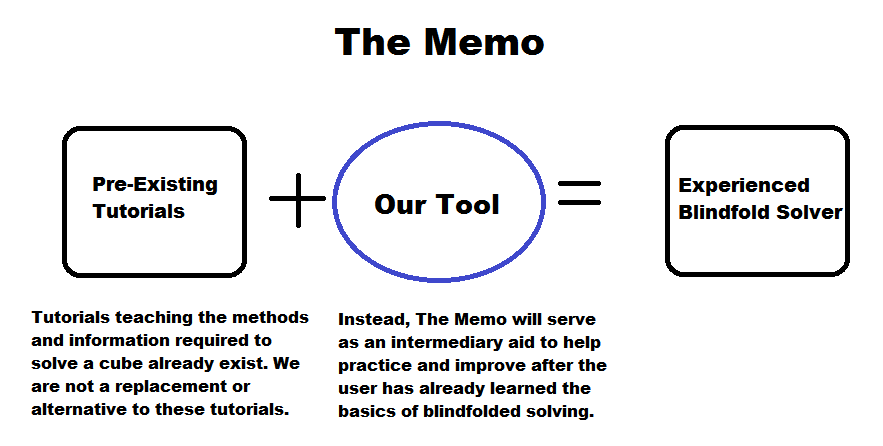
\includegraphics[width = \textwidth]{the_memo_diagram_shit.png}

\par
We will be creating a simple supplementary tool to aid those learning how to solve a 3x3 Rubik’s Cube blindfolded. Creating a web application is the simplest and most accessible form to create this tool and ensure that it’s intuitive to use. We’ll be using CSS and HTML for the organization and appearance of our content and then Javascript will be used to develop the functional aspects of our website and server side code. We don’t need any user data, so we don’t need any database plugins or code. We could expand on our project in this area later if we were to personalize the user experience. \\
\par
Our web application will have four main functions. It will…
\begin{itemize}
\item Show a visual representation of the letters on a virtual Rubik’s Cube.
\item Provide randomly generated scrambles along with corresponding letter solutions.
\item Create the letter strings that correspond to the memorization solution. 
\item Verify user input letter strings to ensure that their solution is correct. 
\end{itemize}
\par
As for non-functional features, we strive to create a tool that is visually pleasing with accurate colors that are clear and visible. We also aim to create a tool that is free of bugs that falls under the WYSIWYG mentality. The goal is to create an intuitive and easy-to-use web application. There will be basic instructions provided, but the user should have no issue or confusion when using our product. We will provide resources for tutorials on the subject as this tool is not a tutorial but rather an aid to practice and improve. \\

\par
As for possible additional features, the first idea is to store user data (success rates, memorization speed, other customizable features, etc.) so we can personalize the user experience. Another feature we could implement is one that generates easy to memorize words for given letter pairs. Example: given the letter pair CT would output an easy to memorize word such as ‘cat’. \\

\section{Use Cases}

\par
The cases of use for this algorithm would be targeted at users who are already familiar at how to solve the Rubik’s cube blindfolded, but need practice. This product that we are developing is aimed primarily as a practice tool for people who cannot fully execute a blindfolded solution to the Rubik’s cube due to memorization failures or algorithm execution. This product would measure the user’s performance and show the points of error(s) in their solution steps or their memorization. \\

\par
The first intended use case of our product is to be a visual tool. We will provide a 3D model of a Rubik’s Cube that is imprinted with their corresponding letters as to which sticker they have. For example, the top left red sticker for the red-blue-white corner could have the letter O (this is not factually accurate, but for the example still stands). Each sticker would then have their own corresponding letter, which can help the user visualize the Rubik’s Cube more easily. We will provide an interface through which the user can examine the cube, and rotate it about on its sides. The rotational property of the cube will be achieved through four orthogonal buttons on a cube face that allow the user to choose which direction to flip the cube 90 degrees. As this is not a truly 3D model but merely a simulated version of a 3D model where only a single face of the Rubik’s cube is shown at a time, we will consider adding “edge” colors that show the colors that are directly on the sides, or edges of the cube so that the user has a frame of reference when performing a rotation on the cube. \\

\par
The second intended use case of our product is to be a memorization tool. Our product will generate a scrambled cube, and then generate the sequence of corresponding letters that correspond to the solution of the cube. The user then has to find a technique to memorize the string of letters in order to solve the Rubik’s Cube. The program will then either verify or correct the user’s solution after memorization; if they memorized correctly, then the program will respond appropriately, but on the other hand, if the user memorized incorrectly, then the program will respond with an incorrect answer and provide the correct string of letters again to refresh the user’s memory, and then present them with an option to try again. As this is working primarily on the memorization skills of the user, it is not necessarily restricted to only Rubik’s Cube users, but to any person who is interested in working on their memorization strength. This is the primary feature of the program, as it is the biggest tool and the biggest aid to help those learn how to solve the Rubik’s Cube blindfolded. It is providing solution strings as a marker for the progress of the user. The scramble can be simpler or longer depending on what the user needs so that if they can only memorize a small chunk at a time then this tool can help them memorize in smaller chunks and gradually learn how to memorize all of the moves. This use case also can appeal to the largest variety of users, which also makes it big in that regard. For a blindfolded Rubik’s Cube solution, it is absolutely essential that the memorization skills of the user is honed in. \\

\par
The third use case for our product is to provide memorization tools to help them form “memorization techniques” to memorize said strings of letters. For example, from a generated scramble, a letter string might be BYOGT - and the program would generate a silly string of words or phrase, such as “Bring Your Own Garbage Tomorrow”. The computer would help the user come up with phrases of strings to help them memorize a random jumble of letters easier. This is the least dynamically functional program of the the three, and we believe the most niche use case of the three as well - we don’t anticipate nearly as many users to have a tough time thinking of word phrases to memorize solving algorithms. It can still be useful as a jump-start for imagination or an example or guide on how to generate phrases to memorize. If a user is really stumped on a string of letters and needs assistance, this third use case can be the answer for their dilemma. Since the scope of this function is so narrow compared to the other user cases, we will be focusing on this feature of the program closer to the end. We will also hold off on the personalization and database features that we mentioned earlier in the ‘Program Description’ section. \\

\par With each use case also comes a potential for bugs and errors. Anywhere where the user interacts with our program, we must ensure that our product does not break; we must make it ‘user-proof’. When considering what errors may arise when the user interacts with our program, it is easy to realize that there are numerous potential errors in the program that can break our algorithm:

\begin{enumerate}
\item The user enters invalid letters that are not on the Rubik’s Cube (for example, the ‘Z’ does not exist on the cube, as there are only 4 * 6, or 24 letters in total for the Cube). We will remedy this by checking if the letter exists on the face of the cube.
\item Cube scrambles result in unsolvable cubes (for example, a red square is duplicated or a square is moved into a position that can no longer be solved). We can remedy this two ways: in one way, the solution will try and solve it and see if it is solvable using backwards checking. In another way, we can guarantee that the cube is not unsolvable by hand-picking each move in a scramble, rather than instantaneously jumping from a solved cube to a scrambled cube.
\item Cube solutions are incorrect or invalid; the algorithm made a mistake (which is easy to happen with so many steps.). We have to implement an algorithm or method that verifies the solution through a second step or an inductive method. There is no clear remedy to this type of error at the moment.
\item User interface is not compatible due to browser; specifically, internet explorer (the least support for browser functionality), or is used on a phone. As an addendum, the webpage must be dynamic in order to fit all types of viewports. This will require heavy research on which CSS and HTML built-in functions have browser supports. We will likely have to avoid webkit functions in order to avoid browser crashes or issues.
\item HTML, CSS, or JS files are hidden, inaccessible, or forbidden (due to permissions), resulting in a loss of functionality, styling, or content from their respective functionalities. This is mostly a file organizational issues. We need to ensure that our files are organized logically and included correctly amongst each other in order to ensure that nothing gets lost. Github can also help us keep track of files, so this one isn’t too big.
\item Variable functionality across different browsers, spontaneous or unpredictable program behavior due to different interfaces. This ties in to point \#4, but doesn’t specifically mean that the browser will crash. We need to ensure that browser behavior across all browsers are identical; we must be careful in which Javascript functions we choose as well.
\item While not necessarily an error, it can be infeasible for the algorithm to take too long to find a solution to a given scrambled cube. Cube scrambling could get stuck in an endless loop or be too inefficient to scramble for a normal human being’s patience. If that is the case, then this is also as big of an issue as any of the others. The remedy for this is to time our program’s runtime and to include engine support for Rubik’s Cube if necessary (and probably a smart idea, too).
\end{enumerate}
\par
There are many other potential bugs that may arise when testing. As reporting for every specific bug would be quite an exhaustive and redundant report, we opted to only include the highest-level and most relevant error cases here. \\

\section{Planning}


\section{Meeting Report}
\par
After the group set up, we have met 3 times on campus.  On our first meeting, we met every members. Every members make brief self introduction to others and set next meeting time. On our second meeting, we settled down majority plan and requirements of our project and designed first version of our project. The frame of our project is came out. In addition, we decided to use google docs for writing and sharing our documents. Using texts, discord and emails for communicate with each other. On this meeting, we separate our project to every group member. Keenan Johnson will working on project description. Jesse Chick will working on planning. Benjamin Martin will working on use cases. Jiaji Sun will working on meeting report. \\

\section{Sources}


\end{document}
